\documentclass[border=1pt]{standalone}
\usepackage{tikz}

% for scaling fonts
\usepackage{scalefnt}
\usepackage{anyfontsize}

\usepackage{xfrac}                     % separated fractions
\usepackage{upgreek}                   % upright greek letters for tau symbol

\definecolor{clepts}{RGB}{51,153,0}	   % A more neutral green
\definecolor{cquarks}{RGB}{90,0,120}   % A more neutral purple
\definecolor{cbosons}{RGB}{153,0,0}	   % Neurtal red, good for dark or light bg
\definecolor{chiggs}{RGB}{204,204,102} % Only for dark BG

% box info function
\newcommand{\leg}[4]{
node[pos=0.5,opacity=1,yshift=9] {\scalefont{0.35}#1}
node[pos=0.5,opacity=1,yshift=3,xshift=6] {\scalefont{0.35}#2}
node[pos=0.5,opacity=1,yshift=-3,xshift=6] {\scalefont{0.35}#3}
node[pos=0.5,opacity=1,yshift=-9] {\scalefont{0.35}#4}
}

% box legend info
\newcommand{\legInit}{
	node[pos=0.5,opacity=1,yshift=9] {\scalefont{0.3}Mass: $\mathrm{eV}/c^2$}
	node[pos=0.5,opacity=1,yshift=3] {\scalefont{0.3}Charge}
	node[pos=0.5,opacity=1,yshift=-3] {\scalefont{0.3}Spin}
	node[pos=0.5,opacity=1,yshift=-9] {\scalefont{0.3}Name}
}

\begin{document}
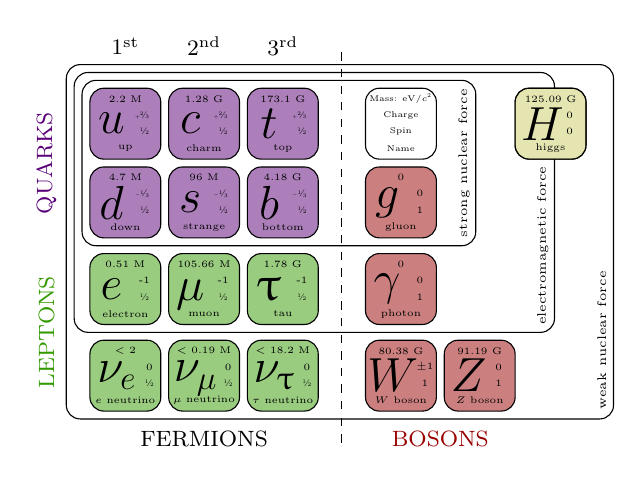
\begin{tikzpicture}[scale=1, every node/.style={transform shape}]

% frame
\draw[rounded corners=5,fill opacity=0] (-0.2,0.2) rectangle (6.75,-4-0.3);
\draw[rounded corners=5,fill opacity=0] (-0.1,0.1) rectangle (6,-3-0.2);
\draw[rounded corners=5,fill opacity=0] (-0.0,0.0) rectangle (5,-2-0.1);

% magenta squares
\draw[rounded corners=5,fill=cquarks,fill opacity=0.5] (0.1,-0.1) rectangle (1,-1) node[pos=0.5,opacity=1,xshift=-5,yshift=0] {\LARGE $u$} \leg{2.2 M}{{$\scriptscriptstyle +$}\sfrac{2}{3}}{\phantom{{$\scriptscriptstyle +$}}\sfrac{1}{2}}{up} node[pos=0.5,opacity=1,yshift=28] {\scalefont{0.8}$1^\mathrm{st}$};
\draw[rounded corners=5,fill=cquarks,fill opacity=0.5] (1+0.1,-0.1) rectangle (1+1,-1)node[pos=0.5,opacity=1,xshift=-5,yshift=0] {\LARGE $c$} \leg{1.28 G}{{$\scriptscriptstyle +$}\sfrac{2}{3}}{\phantom{{$\scriptscriptstyle +$}}\sfrac{1}{2}}{charm} node[pos=0.5,opacity=1,yshift=28] {\scalefont{0.8}$2^\mathrm{nd}$};
\draw[rounded corners=5,fill=cquarks,fill opacity=0.5] (2+0.1,-0.1) rectangle (2+1,-1)node[pos=0.5,opacity=1,xshift=-5] {\LARGE $t$} \leg{173.1 G}{{$\scriptscriptstyle +$}\sfrac{2}{3}}{\phantom{{$\scriptscriptstyle +$}}\sfrac{1}{2}}{top} node[pos=0.5,opacity=1,yshift=28] {\scalefont{0.8}$3^\mathrm{rd}$};
\draw[rounded corners=5,fill=cquarks,fill opacity=0.5] (0.1,-0.1-1) rectangle (1,-1-1)node[pos=0.5,opacity=1,xshift=-5] {\LARGE $d$} \leg{4.7 M}{{$\scriptscriptstyle -$}\sfrac{1}{3}}{\phantom{{$\scriptscriptstyle -$}}\sfrac{1}{2}}{down};
\draw[rounded corners=5,fill=cquarks,fill opacity=0.5] (1+0.1,-0.1-1) rectangle (1+1,-1-1)node[pos=0.5,opacity=1,xshift=-5,yshift=0] {\LARGE $s$} \leg{96 M}{{$\scriptscriptstyle -$}\sfrac{1}{3}}{\phantom{{$\scriptscriptstyle -$}}\sfrac{1}{2}}{strange};
\draw[rounded corners=5,fill=cquarks,fill opacity=0.5] (2+0.1,-0.1-1) rectangle (2+1,-1-1)node[pos=0.5,opacity=1,xshift=-5] {\LARGE $b$} \leg{4.18 G}{{$\scriptscriptstyle -$}\sfrac{1}{3}}{\phantom{{$\scriptscriptstyle -$}}\sfrac{1}{2}}{bottom};

% green squares
\draw[rounded corners=5,fill=clepts,fill opacity=0.5] (0.1,-0.2-2) rectangle (1,-1-2-0.1) node[pos=0.5,opacity=1,xshift=-5,yshift=0] {\LARGE $e$} \leg{0.51 M}{\phantom{{$\scriptscriptstyle +$}}-1}{\phantom{{$\scriptscriptstyle +$}}\sfrac{1}{2}}{electron};
\draw[rounded corners=5,fill=clepts,fill opacity=0.5] (1+0.1,-0.2-2) rectangle (1+1,-1-2-0.1) node[pos=0.5,opacity=1,xshift=-5,yshift=-2] {\LARGE $\mu$} \leg{105.66 M}{\phantom{{$\scriptscriptstyle +$}}-1}{\phantom{{$\scriptscriptstyle +$}}\sfrac{1}{2}}{muon};
\draw[rounded corners=5,fill=clepts,fill opacity=0.5] (2+0.1,-0.2-2) rectangle (2+1,-1-2-0.1) node[pos=0.5,opacity=1,xshift=-5,yshift=0] {\LARGE $\uptau$} \leg{1.78 G}{\phantom{{$\scriptscriptstyle +$}}-1}{\phantom{{$\scriptscriptstyle +$}}\sfrac{1}{2}}{tau};
\draw[rounded corners=5,fill=clepts,fill opacity=0.5] (0.1,-0.3-3) rectangle (1,-1-3-0.2) node[pos=0.5,opacity=1,xshift=-3,yshift=0] {\LARGE $\nu_e$} \leg{< 2}{\phantom{{$\scriptscriptstyle +++$}}0}{\phantom{{$\scriptscriptstyle +++$}}\sfrac{1}{2}}{$e$ neutrino};
\draw[rounded corners=5,fill=clepts,fill opacity=0.5] (1+0.1,-0.3-3) rectangle (1+1,-1-3-0.2) node[pos=0.5,opacity=1,xshift=-3,yshift=-1] {\LARGE $\nu_\mu$} \leg{< 0.19 M}{\phantom{{$\scriptscriptstyle +++$}}0}{\phantom{{$\scriptscriptstyle +++$}}\sfrac{1}{2}}{$\mu$ neutrino};
\draw[rounded corners=5,fill=clepts,fill opacity=0.5] (2+0.1,-0.3-3) rectangle (2+1,-1-3-0.2) node[pos=0.5,opacity=1,xshift=-3,yshift=0] {\LARGE $\nu_\uptau$} \leg{< 18.2 M}{\phantom{{$\scriptscriptstyle +++$}}0}{\phantom{{$\scriptscriptstyle +++$}}\sfrac{1}{2}}{$\tau$ neutrino};

% other squares
\draw[rounded corners=5,fill opacity=0] (3.5 + 0.1, -0.1) rectangle (3.5 + 1, -1)  \legInit;
\draw[rounded corners=5,fill=cbosons,fill opacity=0.5] (3.5 + 0.1, -1 - 0.1) rectangle (3.5 + 1, -2) node[pos=0.5,opacity=1,xshift=-5,yshift=0] {\LARGE $g$} \leg{0}{\phantom{{$\scriptscriptstyle +$}}0}{\phantom{{$\scriptscriptstyle +$}}1}{gluon};
\draw[rounded corners=5,fill=cbosons,fill opacity=0.5] (3.5 + 0.1, -2 - 0.2) rectangle (3.5 + 1, -3 - 0.1) node[pos=0.5,opacity=1,xshift=-5,yshift=0] {\LARGE $\gamma$} \leg{0}{\phantom{{$\scriptscriptstyle +$}}0}{\phantom{{$\scriptscriptstyle +$}}1}{photon};
\draw[rounded corners=5,fill=cbosons,fill opacity=0.5] (3.5 + 0.1, -3 - 0.3) rectangle (3.5 + 1, -4 - 0.2) node[pos=0.5,opacity=1,xshift=-3,yshift=0] {\LARGE $W$} \leg{80.38 G}{\phantom{{$\scriptscriptstyle +++$}}$\pm 1$}{\phantom{{$\scriptscriptstyle +++$}}1}{$W$ boson};
\draw[rounded corners=5,fill=cbosons,fill opacity=0.5] (3.5 + 1 + 0.1, -3 - 0.3) rectangle (3.5 + 2, -4 - 0.2) node[pos=0.5,opacity=1,xshift=-4,yshift=0] {\LARGE $Z$} \leg{91.19 G}{\phantom{{$\scriptscriptstyle +$}}0}{\phantom{{$\scriptscriptstyle +$}}1}{$Z$ boson};
\draw[rounded corners=5,fill=white,fill opacity=1] (4.9 + 1 + 0.1-0.5, -0.1) rectangle (4.9 + 2-0.5, -1);
\draw[rounded corners=5,fill=chiggs,fill opacity=0.5] (4.9 + 1 + 0.1-0.5, -0.1) rectangle (4.9 + 2-0.5, -1) node[pos=0.5,opacity=1,xshift=-3,yshift=0] {\LARGE $H$} \leg{125.09 G}{\phantom{{$\scriptscriptstyle +$}}0}{\phantom{{$\scriptscriptstyle +$}}0}{higgs};


% other stuff
\node[rotate=90] at (5-0.15,-1.05) {\scalefont{0.45}strong nuclear force};
\node[rotate=90] at (6-0.15,-2.1) {\scalefont{0.45}electromagnetic force};
\node[rotate=90] at (7-0.15-0.25,-3.3) {\scalefont{0.45}weak nuclear force};

\node[color=cquarks,rotate=90] at (-0.45,-1.05) {\scalefont{0.8}QUARKS};
\node[color=clepts,rotate=90] at (-0.45,-3.2) {\scalefont{0.8}LEPTONS};
\node[color=black] at (1.55,-4-0.55) {\scalefont{0.8}FERMIONS};
\node[color=cbosons] at (4.55,-4-0.55) {\scalefont{0.8}BOSONS};

% dashed line
\draw[dashed] (3.3,-4-0.6) -- (3.3,0.45) ;

\end{tikzpicture}
\end{document}